
\chapter{Research design}
This chapter contains the information on how the research will be conducted.

\section{Research objective}

\subsection{The problem}
\label{sec:TheProblem}

Right now EFFE is developing an application for employment agencies in which those employment agencies can schedule their employees automatically. To implement custom features that some clients want, EFFE has decided to add something to the business model called building blocks.

\largequote{Building blocks are interchangeable implementations of business logic that can be reused as efficiently as possible}

\subsection{Objective}
The objective is to create a recommendation for an architecture, how to create and maintain such an architecture, where the focus lays on interchangeability and modularity of the different functionalities.

\begin{tabularx}{\linewidth}{|>{\hsize=.3\hsize}X|>{\hsize=.7\hsize}X|}
	\hline
	Stakeholder &
	Interest to the objective
	\\
	\hline
	EFFE &
	EFFE will use this research to enhance its business model. EFFE will also create a better infrastructure which means that the company can implement functionalities faster and cater better to the clients.
	\\
	\hline
	Client &
	The client is not interested in what happens behind the scenes, but the opportunity it brings when partnering with EFFE.
	\\
	\hline
\end{tabularx}

\section{Research framework}

\subsection{Objects}
This chapter describes who/what the objects are for this research and why.

\subsubsection{Backend architecture}
Arguably the most important object is the backend architecture. There are already a great number of researches available regarding backend architecture. The backend is also the place where the business logic will be expressed.

\subsubsection{Frontend architecture}
The second object, frontend architecture, is a lesser known subject when looking at modularity of the actual system. Most of the big companies have a single frontend application per platform.

\subsubsection{Deployment lane}
\label{sec:DeploymentLane}
The backend and the frontend are the software side of the equation but the hardware is also important. The deployment lane is the section that pieces it all together. This object creates the hardware or virtual hardware and sets this hardware up so it can then proceed to deploy the frontend and backend on the just created hardware. How does the current deployment lane change with the new architectures?

\subsubsection{Software architect}
\label{sec:SoftwareArchitect}
The last object to be researched is the software architect. The software architect's job is to design how the system will be build. This can be on a small scale like naming conventions but also bigger scale like layered architecture or modular architecture. Even the programming language can be decided by a software architect.

\subsection{Research perspective}
The research perspective is straight forward. Because this research is written by one of the founders of EFFE it is best to approach this research from the side of EFFE. This means that there will be more emphasis on maintainability than for example performance. Because performance can be bought later on by upgrading hardware but maintainability can only be influenced at the start of a project.

\subsection{Research sources}
This section will describe which sources will be used when evaluating the research objects. This will not include everything but a broad spectrum of the sources that may be used in the research:

\begin{itemize}
	\item \textbf{Modular architecture books: }This research comes down to modular programming. Modular programming is a very broad term and it is important to find how someone else may look at this term.

	\item \textbf{Implementations of modular architectures: }Theory is one side of the coin. Everything can work perfectly in theory but when implementing the theoretic side there will be problems that weren't considered before.

	\item \textbf{Critique from outside: }It is known that software architecture is an opinion based subject. There are no official accepted right way to do certain things. This is because especially this area of software development is fairly young. Software architecture did not have much time to develop itself as much as some other aspects of software engineering such as operating systems. Because software architecture is young there are a great number of people voicing their opinions and it is important to look at the criticism on some of the architectures.

	\item \textbf{Researches on deployment of an architecture: } There will be more than one architecture researched. Each architecture has its own development environment and deployment environment. The infrastructure of the servers on which the program runs is heavily influenced by the architecture of the software.
\end{itemize}

\subsection{Evaluation criteria}
These are the criteria or leading questions that will be asked to research objects. Note: not all evaluation criteria apply to all research objects:

\begin{itemize}
	\item \textbf{What is the biggest pitfall when implementing a new architecture: }As mentioned in \fullref{sec:SoftwareArchitect} the software architect makes the choices around the architecture. So it is important to look at what can go wrong when implementing a new architecture. What are the common pitfalls they have experienced when implementing a new architecture.

	\item \textbf{What are the most used architectures in this area: }There is always a reason why one architecture is very common and the other one isn't. In the research the reasoning will be extracted and reflected on.

	\item \textbf{What are upcoming architectures that are focused on modularity: }Again the whole research is based on the building blocks. These modular functionalities that can be designed via a common interface. What is the difference in solution between these architectures?

	\item \textbf{Which programming languages has the best attributes to complement the modularity: }Some languages are written purely for scripting or some are written to be focused on implementing algorithms more easily. Each programming language has its attributes and which of these attributes are most defining and important to a modular system.

	\item \textbf{Which quality attributes are deemed most important to EFFE?: }The quality attributes from ISO 205010 \cite{iso25010} are the backbone of the architecture. The research will prioritize these quality attributes based on what is most important to EFFE.
\end{itemize}

\subsection{Research framework}

\begin{figure}[H]
	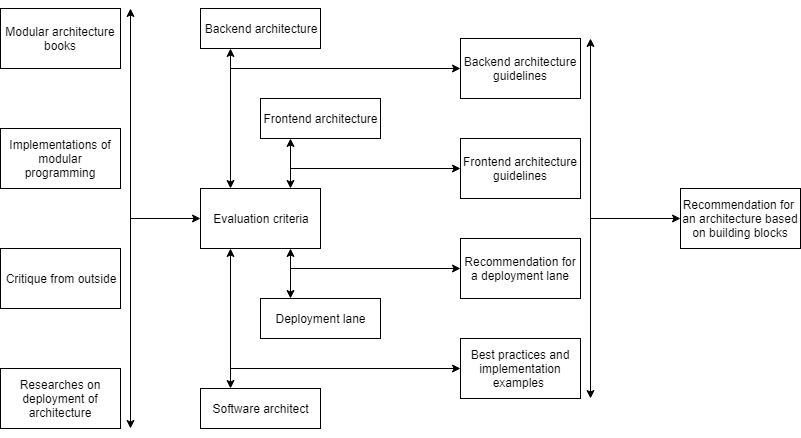
\includegraphics[width=\linewidth]{research_framework.png}
	\caption{Research framework}
\end{figure}

\subsection{Expected Results}
\label{sec:ExpectedResults}

The results will be the guidelines on which the practical part of this research will be based.

\begin{itemize}
	\item \textbf{Backend architecture guidelines: } These are the guidelines on which the backend architecture will be based. These guidelines will indicate why the choice for a certain approach was made and what the specific approach is.

	\item \textbf{Frontend architecture guidelines: } Like with the backend guidelines, these guidelines will also contain the reasoning for each decision made.

	\item \textbf{Recommendation for a deployment lane: } As mentioned in \fullref{sec:DeploymentLane} the deployment lane can impact the backend architecture and vise versa. How does this deployment lane differ from the current deployment lane and why?

	\item \textbf{Best practices and implementation examples: } The software architect's experiences when implementing new architectures together with the implementation of the chosen architecture will conclude in the best practices and the implementation examples.
\end{itemize}

\section{Research Questions}
Note: question 2 and 3 will be handled separately for both backend and frontend.

The main question this research will be answering is:

\largequote{What is the best way to transform a monolith into a modular architecture, where the modules are interchangeable with each other}

\subsection{Question 1}
\label{sec:Question1}
The first question is about software architecture. How does a software architect create a software architecture.

\begin{figure}[H]
	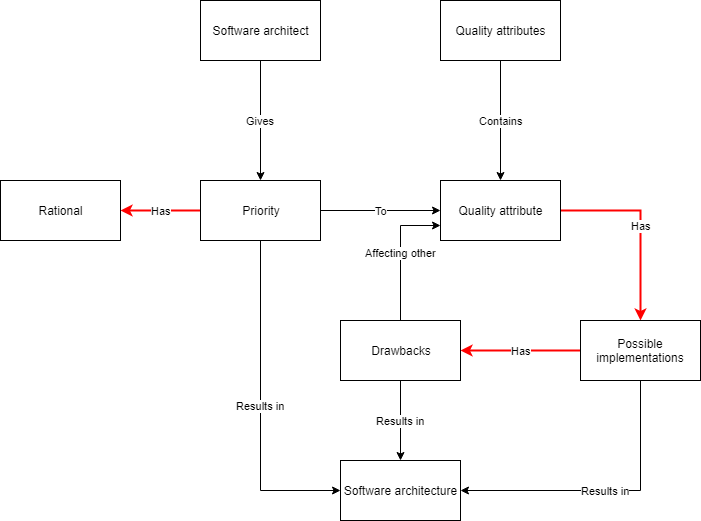
\includegraphics[width=\linewidth]{creating_architecture.png}
        \caption{How a software architecture is chosen}
        \label{fig:ChooseSoftwareArchitecture}
\end{figure}

The red lines show the parts of figure \ref{fig:ChooseSoftwareArchitecture} that will be explored in the question. Thus the question is:

\largequote{What was the thought process behind choosing a software architecture whilst considering each implementation and its quality attributes?}

This question will explore how a software architect chooses their architecture. This will give more insights into what they consider when choosing an implementation so that their rational can be extracted and taken into consideration.

These are some of the sub questions that will be handled based on this central question
\begin{itemize}
	\item Which techniques are used when mapping the priority and the drawbacks in order to make a decision?
	\item How does the priority of a quality attribute influence the end result or software architecture?
	\item How does the software architect combine the priority, drawbacks and possible implementations to a software architecture?
\end{itemize}

\subsection{Question 2}
\label{sec:Question2}
\largequote{What are the best software architectures that mainly focus on modulairty?}

This question focuses on the architectures that are available. The knowledge of how a software architect chooses the architecture is answered in the previous question \fullref{sec:Question1}. Because of the new perspective gained in the previous question there can be a more nuanced choice of architecture.

Sub questions:
\begin{itemize}
	\item What are the up- and downsides of each architecture?
	\item How mature is the documentation and research surrounding the architecture?
	\item Which architecture implements the quality attributes that EFFE deemed important best?
\end{itemize}

\subsection{Question 3}
\largequote{Which implementations are there of the solutions provided for modular architecture?}

The solutions or architectures provided from \fullref{sec:Question2} will have implementations. These implementations may be a theoretic paper or a framework which implements this architecture. This question explores how and why these implementations have been made. Other questions that will be answered are:
\begin{itemize}
	\item How mature is the architecture in contrast to the implementations?
	\item How does the language chosen in the implementation reflect to the architecture?
	\item On what level does the framework compromise which is not reflected in the architecture?
\end{itemize}

\subsection{Question 4}

\largequote{What are the key elements of a software architecture that will influence the deployment lane?}

This question hints at the relation between a software architecture and the deployment lane. Right now there is a limited view on how the deployment lane should be and how it can be. In order for the practical research to work there needs to be an answer to these questions:
\begin{itemize}
	\item Which infrastructure fits best with my chosen architecture?
	\item What are the costs of different infrastructures?
\end{itemize}

\section{Methods}

The methods used to conduct this research will be explained below.

\subsection{Interviews}
The interviews will be conducted with pre-stated questions. These questions may require follow up questions to get a more detailed view. All of the interviews will be recorded and typed out in the \fullref{sec:Interviews}.

\subsection{Desk research}
Most of the research will be desk research. There are lots of studies and small blogs written about the main question. People have shared their experience implementing architectures and their thoughts on it.
